\documentclass[thesis=paper,fancy]{hsmw-thesis}

\title[Inbetreibnahme]{Rock, Paper, Scissors}
\author{Franz Lukas}{Mehlhorn}[B.Eng.]
\addauthor{Robert Swen}{Jehring}[B.Eng.]
\submissiondate{2024}
\email{{fmehlhor@hs-mittweida.de}\and {rjehring@hs-mittweida.de}}


\usepackage{listings}
\usepackage{color}
\usepackage{tabularx}
\usepackage{graphicx}
\usepackage{subcaption}

\bibliographystyle{unsrt}


\definecolor{mygreen}{rgb}{0,0.6,0}
\definecolor{mygray}{rgb}{0.5,0.5,0.5}
\definecolor{mymauve}{rgb}{0.58,0,0.82}

\lstset{ 
  backgroundcolor=\color{white},   % choose the background color; you must add \usepackage{color} or \usepackage{xcolor}; should come as last argument
  basicstyle=\footnotesize,        % the size of the fonts that are used for the code
  breakatwhitespace=false,         % sets if automatic breaks should only happen at whitespace
  breaklines=true,                 % sets automatic line breaking
  captionpos=b,                    % sets the caption-position to bottom
  commentstyle=\color{mygreen},    % comment style
  deletekeywords={...},            % if you want to delete keywords from the given language
  escapeinside={\%*}{*)},          % if you want to add LaTeX within your code
  extendedchars=true,              % lets you use non-ASCII characters; for 8-bits encodings only, does not work with UTF-8
  firstnumber=1,                % start line enumeration with line 1000
  frame=single,	                   % adds a frame around the code
  keepspaces=true,                 % keeps spaces in text, useful for keeping indentation of code (possibly needs columns=flexible)
  keywordstyle=\color{blue},       % keyword style
  language=C++,                 % the language of the code
  morekeywords={*,...},            % if you want to add more keywords to the set
  numbers=left,                    % where to put the line-numbers; possible values are (none, left, right)
  numbersep=5pt,                   % how far the line-numbers are from the code
  numberstyle=\tiny\color{mygray}, % the style that is used for the line-numbers
  rulecolor=\color{black},         % if not set, the frame-color may be changed on line-breaks within not-black text (e.g. comments (green here))
  showspaces=false,                % show spaces everywhere adding particular underscores; it overrides 'showstringspaces'
  showstringspaces=false,          % underline spaces within strings only
  showtabs=false,                  % show tabs within strings adding particular underscores
  stepnumber=2,                    % the step between two line-numbers. If it's 1, each line will be numbered
  stringstyle=\color{mymauve},     % string literal style
  tabsize=2,	                   % sets default tabsize to 2 spaces
  title=\lstname                   % show the filename of files included with \lstinputlisting; also try caption instead of title
}

\begin{document}
\chapter{Einleitung}
In einer zunehmend digitalisierten Welt, in der maschinelles Lernen und künstliche Intelligenz eine immer wichtigere Rolle spielen, gewinnt auch die Anwendung dieser Technologien in Bereichen der Freizeit und des Spiels an Bedeutung. Eine interessante Anwendung dieses Konzepts ist die Entwicklung von Modellen des maschinellen Lernens für Spiele wie Schere, Stein, Papier, die sowohl Unterhaltung bieten als auch als Plattformen für die Erforschung komplexer algorithmischer Konzepte dienen können.
Schere, Stein, Papier ist ein einfaches, jedoch fesselndes Spiel, das seit Generationen von Menschen jeden Alters gespielt wird. Es bietet eine herausfordernde Dynamik, die auf der Annahme basiert, dass die Spieler ihre Handlungen auf unvorhersehbare Weise variieren können, um die Aktionen ihrer Gegner zu schlagen. Diese Eigenschaft macht das Spiel zu einem interessanten Testfall für die Entwicklung und Evaluierung von maschinellen Lernmodellen, die darauf abzielen, die nächste Aktion eines Spielers vorherzusagen und somit eine strategische Grundlage für die Entscheidungsfindung zu schaffen.
Die Arbeit beinhaltet die Untersuchung von Modellen zur Anwendung auf das Schere, Stein, Papier-Spiel. Wir analysieren dabei die vorhandenen Daten und erstellen ein mögliches Modell zum Spielen von Schere, Stein, Papier. Die Effektivität und Genauigkeit der Vorhersage werden dabei ausgewertet. 
Unser Ziel ist es, ein Modell zu entwickeln, das in der Lage ist, die Muster und Trends im Verhalten von Spielern zu erkennen und darauf basierend fundierte Entscheidungen zu treffen. Die Genauigkeit sollte dabei idealerweise mindestens über 33,33\% liegen.

\chapter{Datenanalyse}
\section{Struktur der Daten}
Zu Beginn unseres Projektes muss zuerst die Ausgangssituation geklärt werden. Als Grundlage wird uns ein Datensatz zur Verfügung gestellt, welcher die Ergebnisse eines Schere, Stein, Papier-Spiels zwischen einem Menschen und einem Computer enthält. Die Daten liegen in einer CSV-Datei vor. CSV steht für \glqq Comma-Separated Values\grqq und ist ein einfaches Dateiformat zur Darstellung von tabellarischen Daten. In einer CSV-Datei werden Daten in Zeilen und Spalten organisiert, wobei die Werte durch Kommas voneinander getrennt sind. In selteneren Fällen können auch andere Trennzeichen verwendet werden. Jede Zeile in der Datei repräsentiert einen Datensatz, und die Werte in einer Zeile entsprechen den Spalten. CSV-Dateien sind vergleichsweise einfach zu erstellen und zu verstehen. Sie sind plattformunabhängig und können von verschiedenen Anwendungen und Betriebssystemen verarbeitet werden. Aufgrund ihrer Einfachheit eignen sie sich gut für den Datenaustausch zwischen verschiedenen Systemen. Ein Vorteil von CSV ist sein geringer Speicherbedarf im Vergleich zu binären Formaten oder komplexen Dateitypen. CSV-Dateien sind auch leicht integrierbar. Allerdings fehlt es an Strukturinformationen und Metadaten, was zu Interpretationsproblemen führen kann. CSV ist nicht geeignet für komplexe Datenstrukturen oder große Datensätze, bei denen Datenbanken mit effizienten Abfragemechanismen erforderlich sind. Insgesamt bietet CSV eine einfache Möglichkeit, tabellarische Daten zu speichern und auszutauschen, hat jedoch seine Einschränkungen, insbesondere bei komplexen oder hierarchischen Datenstrukturen. Ein anderer weit verbreiteter Datentyp sind JSON-Dateien. CSV ist im Vergleich zu JSON weniger flexibel, da es keine strukturierte Darstellung für komplexe Datenstrukturen oder hierarchische Informationen bietet. JSON ermöglicht hingegen eine flexible Repräsentation von Daten in verschachtelten Objekten und Arrays. Die Auswahl des geeigneten Formats hängt stark von den Anforderungen der jeweiligen Anwendung ab. Die folgende Abbildung zeigt die zur Verfügung gestellte CSV-Datei.\cite{DeutschneNationalbibliothek.24.04.2023}
\begin{figure}[h]
 		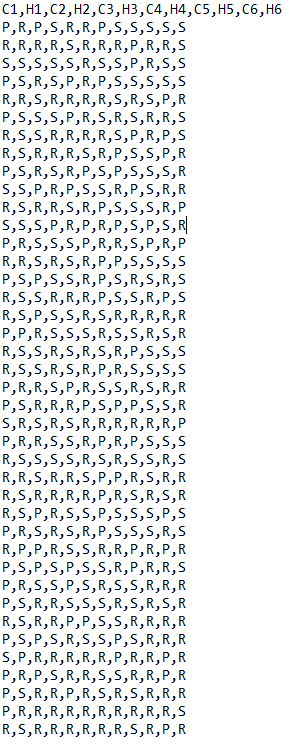
\includegraphics[width=4.5cm, height=7.25cm]{C:/Users/franz/Documents/GitHub/Rock_Paper_Scissors/AIA_Latex/Bilder/CSV_RAW.PNG}
 		\centering
 		\caption{CSV-Datei}
 	\label{fig:CSV-Datei}
\end{figure} 

In der obersten Zeile sind immer abwechselnd H1, C1, H2, C2, …, H6, C6 voneinander getrennt. Man kann sich den Datensatz als Tabelle vorstellen, bei denen H1, C1, H2, C2, …, H6, C6 die Spaltenbezeichner sind. Alle Werte, die in den darunterliegenden Zeilen sind, werden je nach Position einer bestimmten Spalte zugordnet. Die Anordnung als Tabelle wird in der folgenden Tabelle dargestellt.

\begin{figure}[h]
 		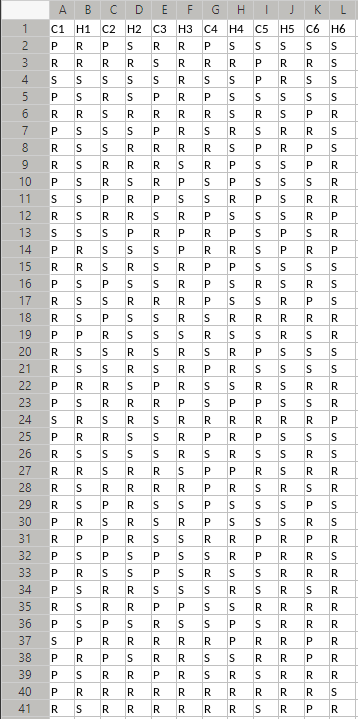
\includegraphics[width=4.5cm, height=7cm]{C:/Users/franz/Documents/GitHub/Rock_Paper_Scissors/AIA_Latex/Bilder/CSV_TAB.PNG}
 		\centering
 		\caption{CSV Datei als Tabelle}
 	\label{fig:CSV Datei als Tabelle}
\end{figure}
Die erste Zeile ist dabei der Bezeichner für die gespielten Spiele. Insgesamt gibt es sechs Runden bei denen immer der Computer gegen den Human (Mensch) spielt. Die zwölf Spalten können somit als sechs Runden interpretiert werden. Jede Runde enthält den Spielzug des Computers und des Humans. Aus der Anzahl der Spalten lässt sich ableiten, dass pro Runde 40 Spiele gespielt wurden. Bei sechs Runden ergibt sich eine insgesamt Spielanzahl von 240 spielen. Durch hinzufügen dieser Metadaten sieht die Tabelle dann wie folgt aus.
\begin{figure}[h]
 		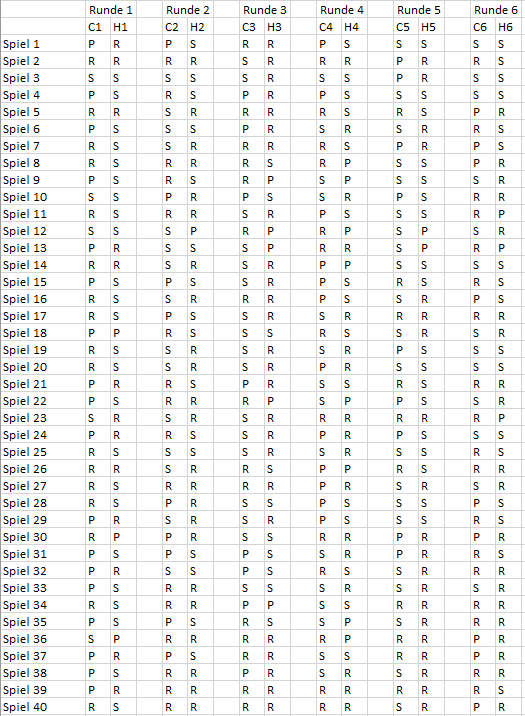
\includegraphics[width=6cm, height=8.5cm]{C:/Users/franz/Documents/GitHub/Rock_Paper_Scissors/AIA_Latex/Bilder/CSV_TAB2.PNG}
 		\centering
 		\caption{CSV Tabelle inklusive Metadaten}
 	\label{fig:CSV Tabelle inklusive Metadaten}
\end{figure}
Das Hinzufügen dieser zusätzlichen Informationen ist für die spätere Verarbeitung mit Hilfe des neuronalen Netzes eher unwichtig. In diesen Schritten geht des darum, die Daten für den Menschen verständlicher zu gestalten. Diese Darstellung sorgt aber für eine höhere Interpretierbarkeit und ermöglicht eine statistische Analyse der Daten. Diese ist vor allem für die spätere Modellentwicklung wichtig. Auf die statistische Analyse und Visualisierung der Daten wird im folgenden Teil eingegangen.
\section{Statistische Analyse und Datenvisualisierung}
Auf Grund der zusätzlich gewonnenen Informationen der Daten ist es möglich eine erste statistische Analyse durchzuführen. In diesem Abschnitt wird nur auf einen Teil der Analyse eingegangen, welcher sich mit Abbildungen zusätzlich gut visualisieren lässt. 
Der erste Punkt der Analyse ist die Ergebnisverteilung der Spiele. Also wie oft hat der Mensch, wie oft hat der Computer gewonnen und wie oft ist eine Runde als Unentschieden ausgegangen ist.
\begin{figure}[h]
 		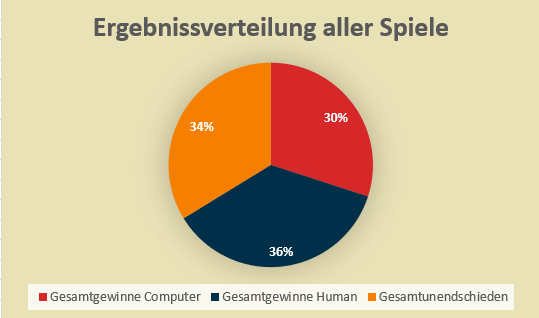
\includegraphics[width=7cm, height=4cm]{C:/Users/franz/Documents/GitHub/Rock_Paper_Scissors/AIA_Latex/Bilder/Abb1.PNG}
 		\centering
 		\caption{Ergebnisverteilung aller Spiele}
 	\label{fig:Ergebnisverteilung aller Spiele}
\end{figure}

Wie in der Abbildung zu sehen hat der Mensch 36\% der Spiele gewonnen, der Computer 30\% und zu 34\% ist das Spiel Unentschieden ausgegangen. Wären die Ergebnisse gleichverteilt hätte jede Möglichkeit eine Wahrscheinlichkeit von 33,33 \% erhalten müssen. Wie zu erkennen sind die Ergebnisse relativ nah an einer Gleichverteilung. Was die gewonnenen Spiele an geht, hat der Mensch etwas die überhand gegenüber dem Computer.
Die einzelnen runden sehen der Gesamtverteilung sehr ähnlich. Lediglich die Runden 1 und 3 sind einzelne Ausreißer.

\begin{figure}[h]
   \begin{minipage}[b]{.45\linewidth} % [b] => Ausrichtung an \caption
      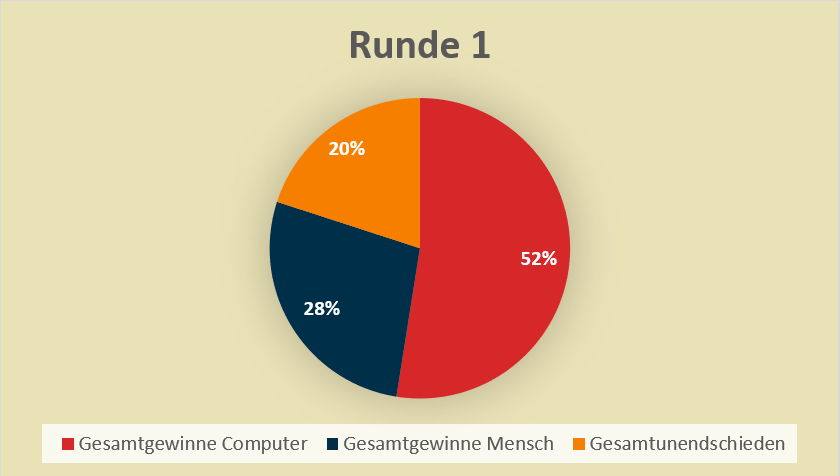
\includegraphics[width=\linewidth]{C:/Users/franz/Documents/GitHub/Rock_Paper_Scissors/AIA_Latex/Bilder/Abb2.PNG}
      \caption{Ergebnisse Runde 1}
   \end{minipage}
   \hspace{.1\linewidth}% Abstand zwischen Bilder
   \begin{minipage}[b]{.45\linewidth} % [b] => Ausrichtung an \caption
      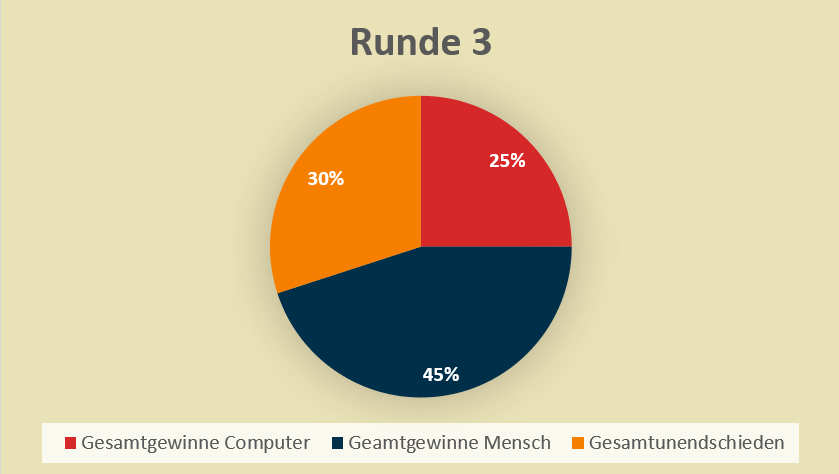
\includegraphics[width=\linewidth]{C:/Users/franz/Documents/GitHub/Rock_Paper_Scissors/AIA_Latex/Bilder/Abb3.PNG}
      \caption{Ergebnisse Runde 3}
   \end{minipage}
\end{figure}
In Runde 1 hat der Computer 52\% der Spiele gewonnen. In Runde 3 dagegen hat der Mensch wieder ein besseres Spiel und gewinnt mit 45\% fast jedes zweite Spiel. Über die genauen Gründe für diese Ergebnisse lassen sich nur Vermutungen anstellen. In der ersten Runde spielt der Mensch fast ausschließlich Scissors und zweimal Paper. Wie oft eine bestimmte Möglichkeit gespielt wurde, ist ebenfalls Teil der Analyse. Die nächsten vier Abbildungen zeigen, welche Möglichkeiten durch den Computer gewählt wurden und mit welcher Wahrscheinlichkeit er damit gewonnen hat.
\begin{figure}[h]
   \begin{minipage}[b]{.45\linewidth} % [b] => Ausrichtung an \caption
      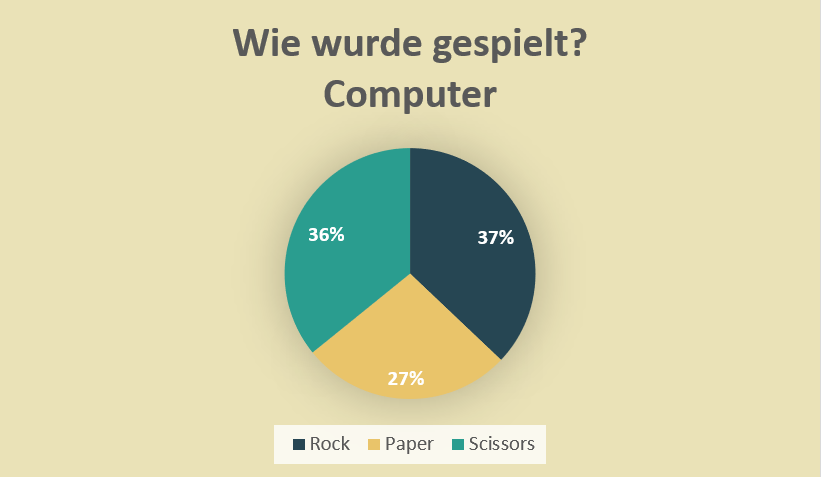
\includegraphics[width=\linewidth]{C:/Users/franz/Documents/GitHub/Rock_Paper_Scissors/AIA_Latex/Bilder/Abb4.PNG}
      \caption{Spielzüge Computer}
   \end{minipage}
   \hspace{.1\linewidth}% Abstand zwischen Bilder
   \begin{minipage}[b]{.45\linewidth} % [b] => Ausrichtung an \caption
      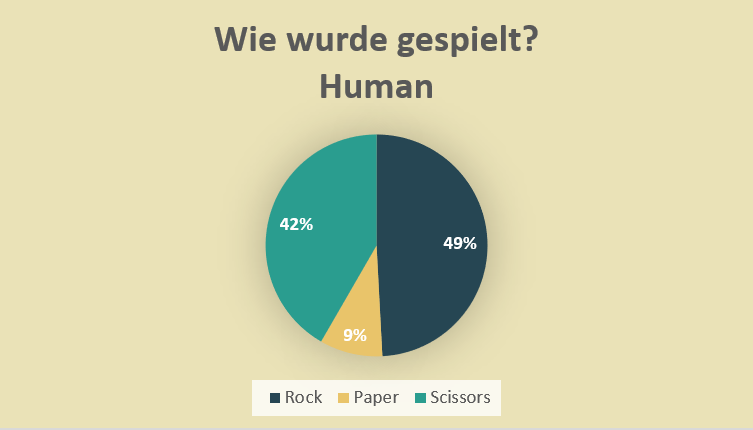
\includegraphics[width=\linewidth]{C:/Users/franz/Documents/GitHub/Rock_Paper_Scissors/AIA_Latex/Bilder/Abb5.PNG}
      \caption{Spielzüge Mensch}
   \end{minipage}
\end{figure}
\begin{figure}[h]
   \begin{minipage}[b]{.45\linewidth} % [b] => Ausrichtung an \caption
      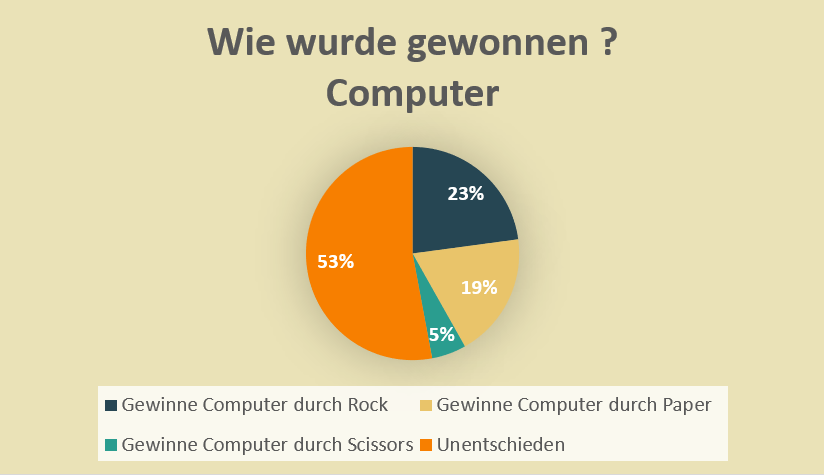
\includegraphics[width=\linewidth]{C:/Users/franz/Documents/GitHub/Rock_Paper_Scissors/AIA_Latex/Bilder/Abb6.PNG}
      \caption{Gewinne Computer}
   \end{minipage}
   \hspace{.1\linewidth}% Abstand zwischen Bilder
   \begin{minipage}[b]{.45\linewidth} % [b] => Ausrichtung an \caption
      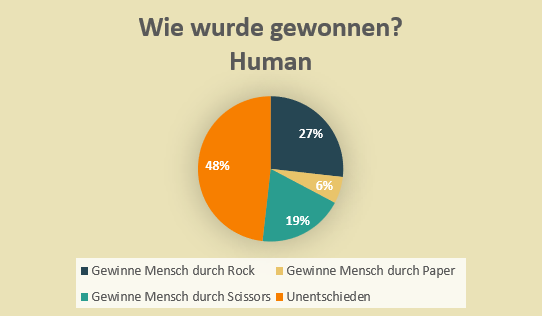
\includegraphics[width=\linewidth]{C:/Users/franz/Documents/GitHub/Rock_Paper_Scissors/AIA_Latex/Bilder/Abb7.PNG}
      \caption{Gewinne Mensch}
   \end{minipage}
\end{figure}

In den Abbildungen der gewonnenen Spiele wurden die Spiele, welche unentschieden ausgegangen sind, ebenfalls mit Berücksichtigt. Anderenfalls würden die resultierenden Prozentwerte schlecht zu vergleichen sein.
Hier lässt sich wieder erkennen, dass die Spielzüge relativ gleichverteilt sind. Lediglich Paper wurde mit 27\% ca. 10\% weniger gespielt als Rock oder Scissors. Die Abbildungen, mit welchen Möglichkeiten gewonnen wurde, sieht weniger gleichverteilt aus. Zu Beginn ist zu erkennen, dass ca. 50\% der Spiele für den Computer und Mensch untenschieden ausgegangen sind. Beim Computer wurden fast die Hälfte der Siege (23\% Prozent in der Gesamtwertung mit Unentschieden) über Rock erspielt. Ebenso groß ist Paper mit 19\% der Siege. Dementsprechend ist Scissors mit nur 5\% unterrepräsentiert. Diese Ergebnisse hängen natürlichen mit den gespielten Möglichkeiten des Menschen zusammen. Wir die nächste Abbildung zeigt, hat der Mensch lediglich 9\% der Spiele die Möglichkeit Paper gewählt.
Aus diesem Grund kann der Computer auch nur so wenige Spiele mit Scissors gewinnen. Der einzige Weg mit Scissors zu gewinnen, ist gegen Paper zu spielen, wird das aber durch den Gegner so gut wie nie gespielt, ist das Gewinnen um so unwahrscheinlicher. Durch diese Diagramme lässt sich relativ gut die Korrelation zwischen den gespielten Möglichkeiten erkennen. Ein Auffälliger Fakt ist, dass der Mensch nach einer gewonnenen Runde meist eine andere Möglichkeit spielt. Bei Runden, die unentschieden ausgehen bleibt der Mensch sich meist treu und spielt die Möglichkeit erneut.

\chapter{Modelldesign}

\section{Datencodierung}
Eine Möglichkeit zur Kodierung der Daten ist das One-Hot-Encoding. 
One-Hot-Encoding ist eine Technik zur Kodierung von kategorialen Variablen in einem maschinenlesbaren Format. Es wird häufig in Machine-Learning-Anwendungen verwendet, insbesondere wenn die Eingabedaten kategorische Merkmale enthalten, die nicht direkt in numerischen Formen vorliegen. Die Idee hinter One-Hot-Encoding besteht darin, jede Kategorie in eine binäre Vektorrepräsentation umzuwandeln, bei der jede Dimension des Vektors einem möglichen Wert der kategorialen Variable entspricht. Eine Dimension wird auf 1 gesetzt, wenn der Wert der kategorialen Variable mit dieser Dimension übereinstimmt, und auf 0 gesetzt, wenn nicht.
Hier ist ein einfaches Beispiel: \\
Angenommen, wir haben eine kategoriale Variable Farbe mit den möglichen Werten Rot, Grün und Blau. Mit One-Hot-Encoding würden wir diese in drei binäre Merkmale umwandeln:

\begin{itemize}
\item Rot wird zu [1, 0, 0]
\item Grün wird zu [0, 1, 0]
\item Blau wird zu [0, 0, 1]
\end{itemize}
Durch diese Umwandlung wird vermieden, dass das Modell annimmt, dass es eine Rangordnung oder eine quantitative Beziehung zwischen den verschiedenen Kategorien gibt. Die genaue Umsetzung der One-Hot-Kodierung in unserem Schere, Stein, Papier Beispiel wird im Kapitel 3.2 betrachtet.


\section{Mögliche Modelle}
Zur Vorhersage der nächsten Auswahl eines Spielers in einem Stein-Schere-Papier-Spiel gibt es unzählige verschiedene Möglichkeiten. Einige mögliche Modelle wurden in den nachfolgenden Punkten aufgelistet. Dabei handelt es sich nur um eine Auswahl möglicher Modelle:

\begin{itemize}
	\item [1.] Entscheidet sich für die Option, die entweder gegen die vorherige Wahl des Spielers verlieren oder sie schlagen würde. Die Annahme hierbei ist, dass ein Spieler seine vorherigen Entscheidungen entweder nicht wiederholt oder wiederholen wird.
	\item [2.] Nutzt eine vektorbasierte Auswahl basierend auf den letzten drei Runden. Die Annahme hierbei ist, dass ein Spieler ein bestimmtes Muster verwendet, wie zum Beispiel Stein, Papier, Schere, Stein, Papier, Schere usw.
	\item [3.] Entscheidet sich für die Option, die die häufigste letzte Wahl des Spielers schlagen würde. Die Annahme ist, dass ein Spieler eine bestimmte Wahl hat, die er häufig wiederholt.
	\item [4.] Entscheidet sich für die Option, die die am seltensten gespielte Wahl des Spielers schlagen würde. Die Annahme ist, dass der Spieler versucht, die Wahl zu spielen, die er schon lange nicht mehr gespielt hat.
	\item [5.] Nutzt ein auf historischen Daten trainiertes neuronales Netzwerkmodell von Scikit-Learn. Es soll die nächste Wahl des Spielers auf der Grundlage der Daten der letzten 7 Runden vorhersagen und schlagen.
	\item [6.] Nutzt ein auf historischen Daten trainiertes Entscheidungsbaummodell von Scikit-Learn. Es soll die nächste Wahl des Spielers auf der Grundlage der Daten der letzten 5 Runden vorhersagen und schlagen.  
\end{itemize}

Jedes dieser Modelle basiert auf unterschiedlichen Annahmen und Strategien, um die nächste Auswahl eines Spielers vorherzusagen. Je nach den Spielgewohnheiten und Mustern des Spielers können verschiedene Modelle unterschiedlich gut funktionieren. \cite{AustinFischer.2021}
Wie das Modell für diese Beispielaufgabe aufgebaut ist, wird im Kapitel 3.3 genauer beschrieben.

\chapter{Umsetzung}

\section{Vorbereitung}
Für die Erstellung des Maschine Learning Models wird in dieser Arbeit ein Jupyter Notebook verwendet, um die einzelnen Teilschritte separat voneinander ausführen zu können und damit auch Änderungen am Model zu erleichtern. Bevor es zur eigentlichen Implementierung in Python kommen kann, sind zunächst einige Installationen notwendig. Die \glqq Graphviz\grqq{} ist dabei ein optionales System-Packet, welches grundsätzlich zur Visualisierung von Objekten und deren Beziehungen untereinander dient. Es visualisiert somit gerichtete und ungerichtete Graphen. In dieser Arbeit wird es konkret zur Visualisierung des neuronalen Netztes beziehungsweise dessen Layer verwendet. Nicht optional sind hingegen die Python Python-Pakete \glqq tensorflow \grqq, \glqq keras\grqq, \glqq numpy\grqq, \glqq pandas\grqq und \glqq{} scikit-learn\grqq{} , welche über das Python Paketverwaltungsprogramm pip installiert werden.

\section{Datenverarbeitung und Implementierung}
Nach dem Import der im Vorbereitungsteil genannten Pakete beginnt die Implementierung mit dem Einlesen der bereitgestellten CSV-Datei als sogenanntes Pandas-Dataframe und der Berechnung der Dimension dieses Dataframes. Die Daten beziehungsweise die Stein-Schere-Papier-Spiele sind hierbei in sechs Gruppen oder Spiel-Sets mit je 40 Spielen gegliedert. Aus diesem Grund werden im nächsten Schritt diese sechs Sets als separate Dataframes selektiert und in ein Array eingelesen. Danach erfolgt für jedes dieser Spiel-Sets die Bestimmung des Gewinners der 40 enthaltenen Spiele, da dies für die späteren Input-Layer des Models wichtig wird. Es wird hierzu betrachtet, ob der Spieler (\glqq H\grqq -Human) gegen die zufallsgenerierten Werte (\glqq C\grqq - Computer) gewonnen, verloren oder unentschieden gespielt hat. Bei einem Sieg wird der Wert 1, bei einer Niederlage der Wert -1 und bei einem Unentschieden der Wert 0 vergeben. Im Anschluss daran folgt das Data-Encoding über die Initialisierung eines One-Hot-Encoders und der Datencodierung des initial aus der CSV-Datei eingelesenen Dataframes. Der One-Hot-Encoder erzeugt hierzu über die \glqq fit\grqq-Methode selbst die Encoder-Kategorien, welche in diesem Fall dem Array ['P', 'R', 'S'] entsprechen. Die Reihenfolge der Kategorien in diesem Array ist dabei entscheidend für die Datencodierung. Ein 'R' im Dataframe wird so beispielsweise zu [0., 1., 0.] one-hot-codiert. Das one-hot-codierte Dataframe wird daraufhin zur weiteren Verarbeitung erneut in ein Array bestehend aus den sechs Spiel-Sets zerlegt. Nach diesem Schritt können die Spiel-Sets mit dem entsprechenden Gewinner-Array über die \glqq concat“-Methode des Pandas-Python-Pakets zusammengefügt werden. Ein Row eines der Sets entspricht damit zum Beispiel [[1.0, 0.0, 0.0], [0.0, 1.0, 0.0], -1], was original-codiert wiederum ['P', 'R', 'verloren'] entsprechen würde. Aus diesen Datensätzen lassen sich jetzt die Trainings- und die Validierungsdatensätze erstellen. Dabei ist es zunächst notwendig, das Verhältnis zwischen Trainings- und Validierungsdaten festzulegen. Dieses Verhältnis gibt an, wieviel Rows jedes der sechs Spiel-Sets für das Training und wie viele für dessen Validierung verwendet werden. Für die hier vorliegende Lernaufgabe wird aufgrund des vergleichsweisen kleinen Gesamtdatensatzes von insgesamt 240 Spielen ein 70:30 Verhältnis angewendet. Das resultiert somit in 28 Trainings-Rows beziehungsweise 12 Validierungs-Rows pro Spiel-Set, also 168 Spiele für das Training und 72 Spiele für die Validierung. Die Trennung zischen Trainings- und Validierungsdatensätzen entlang der X-Achse des Original-Dataframes der CSV-Datei ist dabei beabsichtigt gewählt, um Trainings- und Validierungsdaten aus allen sechs Spiel-Sets zu erhalten. So soll vermieden werden, dass im Falle einer vertikalen Trennung (also beispielsweise Spiel-Set 1-5 als Training und Spiel-Set 6 als Validierung) sich eines der Spiel-Sets signifikant von den anderen unterscheidet und dadurch das Training oder die Validierung negativ beeinflusst (biased) wird. Nach dieser Trennung müssen die sechs Trainings- und sechs Validierungssets für die Verwendung im Model jeweils zu einem Trainings- und einem Validierungs-Dataframe zusammengeführt werden.

\section{Model-Design}
Grundlegend besteht das für die hier vorliegende Lernaufgabe verwendetet neuronale Netz aus zwei Input-Layern, zwei vollvernetzten (dense) Hidden-Layern und einem Output-Layer. Die beiden Input-Layer ergeben sich aus der Struktur der beschriebenen Trainings- und Validierungsdatensätzen, welche jeweils aus einem Array mit drei Werten und einem Array mit einem Werte bestehen. Die beiden folgenden Dense-Layer besitzen eine Output-Dimension von 64 und verwenden die sogenannte 
Code	Ausgabe \glqq ReLu\grqq{}-Aktivierungsfunktion. Der für die Ausgabe der Wahrscheinlichkeiten für Stein, Schere und Papier dreidimensionale Output-Layer verfügt wiederum über die „Softmax\grqq -Aktivierungsfunktion. Als \glqq Loss\grqq{} wird die \glqq Categorical Crossentropy\grqq{} und als \glqq Optimizer\grqq{} der Adam Algorithmus des Keras Pakets verwendet. Somit soll das Ziel des Models sein, den nächsten Zug beziehungsweise die nächste Wahl des Spielers zwischen den drei Möglichkeiten Stein, Schere und Papier vorherzusagen. Dies soll dabei auf Basis des letzten Spiels beruhen, also auf der letzten Auswahl des Spielers und ob er damit gewonnen hat oder nicht. Um das Model dahingehend zu trainieren, ist es notwendig aus den Trainings- und Validierungsdatensätze einen X- und einen Y-Datensatz zu erstellen. Der X-Datensatz entspricht dabei dem originalen Trainings- beziehungsweise Validierungsdatensatz. Der Y-Datensatz entspricht wiederum dem jeweiligen originalen Datensatz dessen Row-Index um plus eins verschoben ist. Im Anschluss daran wird das Model mit diesen X- und Y-Datensätzen bei einer Batch-Size von 32 für 10 Epochen trainiert und validiert. Es entsteht so eine Accuracy der Vorhersage des nächsten Zuges von rund 50\% (49,40\%). Dieser Wert lässt sich durch weiteres Testen Modifizieren am Model sicher noch stark verbessern.

\chapter{Fazit}
Die vorliegende Arbeit hat einen Einblick in die Anwendung von maschinellem Lernen auf das Schere, Stein, Papier-Spiel geboten und verschiedene Modellansätze genannt. Ein Modellansatz wurde dabei als Beispiel verwendet und in einem Jupyter Notebook umgesetzt. Unsere Ergebnisse zeigen, dass maschinelle Lernmodelle potenziell in der Lage sind, die Muster und Trends im Verhalten von Spielern zu erkennen und somit fundierte Entscheidungen zu treffen. Wir haben festgestellt, dass Modelle, die auf neuronalen Netzwerken basieren, eine hohe Vorhersagegenauigkeit erreichen können, insbesondere wenn sie mit ausreichend Trainingsdaten und sorgfältiger Modellierung trainiert werden.
Dennoch ist anzumerken, dass die Vorhersage der nächsten Aktion in einem dynamischen und unvorhersehbaren Spiel wie Schere, Stein, Papier herausfordernd bleibt, da menschliche Spieler in der Lage sind, ihre Strategien spontan anzupassen und zu variieren. Es bleibt daher eine interessante Herausforderung für zukünftige Forschung, die Leistungsfähigkeit dieser Modelle weiter zu verbessern und zu verfeinern, um eine breitere Anwendbarkeit und Robustheit zu gewährleisten.


\bibliography{Literautur}
	
\end{document}
